% Drawing 146/03-6 -- folder 146, batch 03, archive page 59 (PDF page 60).
% Transcription: en bas, plusieurs croquis largement raturés : une ellipse, une sphère en fuseaux à quatre sommets cerclés (« $9 = 5 + 4\,\struck{+1}$ sommets », « 30 possibilités (car il faut choisir l'orientation du carré) »), une petite sphère à quatre sommets, un tétraèdre, une sphère « $D_1$ » ; flèches « $\to D_1$ », « $\mathbb{Z}$ ». À gauche, une liste :
% Kind: struck sketches (spheres, tetrahedron). Method 2 (schematic redraw from the facsimile). Status: partial.
% Notes: Strike-outs are not drawn (issue 128). Struck in the original and left out: the ellipse (crossed by a zigzag), the sphere in lunes with four ringed vertices (crossed by long diagonal strokes), the tetrahedron (crossed by a zigzag) and the sphere at the bottom right (scribbled over), the « +1 » of « 9 = 5 + 4 + 1 sommets ». Drawn: the small sphere with its top vertex and four ringed vertices on the equator (back half pencil), joined to the top vertex by four arcs; the arrow « -> D1 », the second arrow with « Z » as the transcription reads it (the « Z » may be the start of the zigzag over the tetrahedron), the legends « 9 = 5 + 4 sommets », « 30 possibilités (car il faut choisir l'orientation du carré) », which are not struck, and the label D1 at the right, which belonged to the struck sphere. The list on the left (D0 -> D1 ...) is text, carried by the transcription. Still differs: the small sphere's arcs are smooth curves read by eye; whether its outline is closed at the lower right is unclear. Redrawn 2026-11-09 (issue 128): to check again. Question settled by a machine pass on the facsimile, 2026-11-12 (page): the ellipse and the tetrahedron are each crossed by a zigzag, the sphere in lunes by long oblique strokes and the bottom right sphere by a scribble: all four are struck and stay left out. The sign after the arrows is a heavy Z with a doubled stroke, in a heavier pen than the thin zigzag over the tetrahedron and apart from it: a letter, kept. Not checked by a reader. 2026-11-13, Claude Opus 5.5, overlay check (issue 147): rasterised from its own coordinates over the 400 dpi colour scan (250 ppi native) on a unit grid; not compiled (no TeX in the session). The small sphere, its arcs and ringed vertices, the two arrows and the legends lie on their ink to within about 1 unit. Changed, following the editor's rule for wholly struck figures (#146: what lies under the strike is drawn, and the figure is recorded as struck): the four struck sketches are now drawn in the struck style, as far as they can be read under the strokes that cross them: the ellipse; the sphere in lunes (outline, front equator and dashed back, the ring at the top, four arcs from it to the four ringed vertices on the equator); the tetrahedron (four ringed vertices, the edges from the top to the left, right and bottom vertices, the left and right edges down to the bottom vertex, and the dashed stroke from the left vertex to a fourth ringed point inside); the sphere at the bottom right (outline, ring at the top, the vertical meridian, the equator and four ringed points). The zigzags, diagonal strokes and scribbles that cross them are left out (crossings-out are not figures). Still differs: under the crossings-out, the edges of the tetrahedron and the inner strokes of the two struck spheres are a reading and lie within 1 to 2 units of the ink; the small sphere's arcs are smooth curves, and whether its outline is closed at the lower right is unclear.
% Coordinates: 1 unit = 1 mm = 1/100 of the crop width (bbox in page fractions: [0.08, 0.64, 0.95, 0.88]).
% Redrawn by Claude (claude-opus-5-5), issue #73, 2026-11-09; not checked by a human; not compiled (no TeX in the session).
% Checked by Claude (claude-opus-5-5) 2026-11-13 (issue #147): overlaid on the 400 dpi colour facsimile; not compiled (no TeX in the session). Not checked by a human. Status: partial.
% Rights: reproduces part of the work -- behind RENDER_TRANSCRIPTS, never published by itself.
\documentclass[tikz,border=3pt]{standalone}
\usepackage{amsmath,amssymb}
\usetikzlibrary{patterns,arrows.meta}
\tikzset{pencil/.style={black!45}, struck/.style={black!35}, mark/.style={circle,draw,inner sep=1.3pt}, pt/.style={circle,fill,inner sep=0.9pt}, opt/.style={circle,draw,fill=white,inner sep=1.1pt}}
\begin{document}
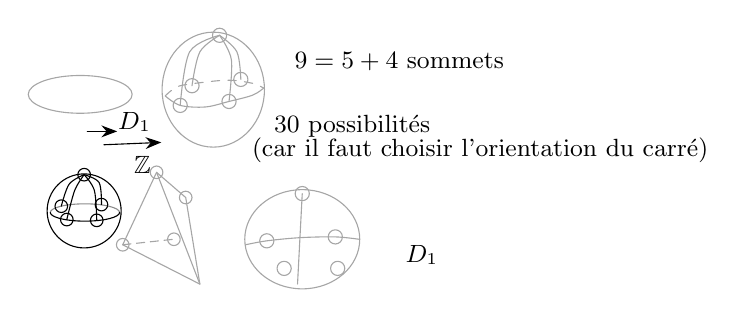
\begin{tikzpicture}[x=1mm,y=1mm,line cap=round,line join=round,font=\scriptsize]
\draw[struck] (44.6,-11.4) ellipse[x radius=6.6, y radius=2.4];
\draw[struck] (61.5,-10.8) ellipse[x radius=6.5, y radius=7.3];
\draw[struck] plot[smooth, tension=0.55] coordinates {(55.4,-11.6) (57.3,-12.8) (60.5,-13) (63.5,-12.3) (66.5,-11.5) (67.9,-10.6)};
\draw[struck,dashed] plot[smooth, tension=0.55] coordinates {(55.4,-11.6) (57,-10.4) (60,-9.9) (63.5,-9.6) (66.5,-10) (67.9,-10.6)};
\draw[struck] (62.3,-3.9) circle[radius=0.9];
\draw[struck] plot[smooth, tension=0.55] coordinates {(62.3,-3.9) (58.5,-6) (57.3,-12.8)};
\draw[struck] plot[smooth, tension=0.55] coordinates {(62.3,-3.9) (59.8,-6) (58.8,-10.3)};
\draw[struck] plot[smooth, tension=0.55] coordinates {(62.3,-3.9) (64.5,-6) (65,-9.5)};
\draw[struck] plot[smooth, tension=0.55] coordinates {(62.3,-3.9) (63.8,-7) (63.5,-12.3)};
\draw[struck] (57.3,-12.8) circle[radius=0.9];
\draw[struck] (58.8,-10.3) circle[radius=0.9];
\draw[struck] (65,-9.5) circle[radius=0.9];
\draw[struck] (63.5,-12.3) circle[radius=0.9];
\draw[struck] (54.3,-21.3) -- (50,-30.5) -- (59.8,-35.5) -- (58,-24.5) -- cycle;
\draw[struck] (54.3,-21.3) -- (59.8,-35.5);
\draw[struck,densely dashed] (50,-30.5) -- (56.5,-29.8);
\draw[struck] (54.3,-21.3) circle[radius=0.8];
\draw[struck] (58,-24.5) circle[radius=0.8];
\draw[struck] (50,-30.5) circle[radius=0.8];
\draw[struck] (56.5,-29.8) circle[radius=0.8];
\draw[struck] (72.8,-29.8) ellipse[x radius=7.3, y radius=6.3];
\draw[struck] (72.8,-24) circle[radius=0.9];
\draw[struck] (72.8,-24) -- (72.2,-35.5);
\draw[struck] plot[smooth, tension=0.55] coordinates {(65.6,-30.5) (68.3,-30) (72.5,-29.6) (77,-29.5) (80,-29.8)};
\draw[struck] (68.3,-30) circle[radius=0.9];
\draw[struck] (77,-29.5) circle[radius=0.9];
\draw[struck] (70.5,-33.5) circle[radius=0.9];
\draw[struck] (77.3,-33.5) circle[radius=0.9];
\draw (45.1,-26.2) circle[radius=4.7];
\draw[pencil] (49.6,-26.4) arc[start angle=0, end angle=180, x radius=4.4, y radius=1.1];
\draw (40.8,-26.4) arc[start angle=180, end angle=360, x radius=4.4, y radius=1.1];
\draw plot[smooth, tension=0.55] coordinates {(45.1,-21.6) (43.2,-22.8) (42.2,-25.6)};
\draw plot[smooth, tension=0.55] coordinates {(45.1,-21.6) (47,-22.6) (47.3,-25.4)};
\draw plot[smooth, tension=0.55] coordinates {(45.1,-21.6) (43.9,-23.6) (42.9,-27.3)};
\draw plot[smooth, tension=0.55] coordinates {(45.1,-21.6) (46.4,-23.6) (46.7,-27.4)};
\draw (45.1,-21.6) circle[radius=0.8];
\draw (42.2,-25.6) circle[radius=0.8];
\draw (47.3,-25.4) circle[radius=0.8];
\draw (42.9,-27.3) circle[radius=0.8];
\draw (46.7,-27.4) circle[radius=0.8];
\draw[-{Stealth[length=2mm]}] (45.5,-16.1) -- (49.3,-16.1);
\node[inner sep=1pt] at (51.5,-14.9) {\small $D_1$};
\draw[-{Stealth[length=2mm]}] (47.6,-17.8) -- (54.9,-17.5);
\node[inner sep=1pt] at (52.5,-20.4) {\small $\mathbb{Z}$};
\node[inner sep=1pt,anchor=west] at (71.4,-7.2) {\small $9 = 5+4$ sommets};
\node[inner sep=1pt,anchor=west] at (68.8,-15.5) {\small 30 possibilités};
\node[inner sep=1pt,anchor=west] at (66,-18.5) {\small (car il faut choisir l'orientation du carré)};
\node[inner sep=1pt] at (88,-31.8) {\small $D_1$};
\end{tikzpicture}
\end{document}
